\chapter{Koja \v{z}ivotinja nam je donela SARS?}
\setbookcodestyle

\section{Uvod}
\label{sec:uvod}

Neka od glavnih pitanja koja mo\v{z}emo postaviti su:
Koja \v{z}ivotinja nam je donela SARS? Kako smo se prvobitno zarazili? Kako se SARS \v{s}irio po svetu? Sva ova pitanja spadaju u domen filogenetske analize koja se bavi rekonstrukcijom evolutivnih stabala.

\section{Izbijanje epidemije}
\label{sec:izbijanjeepidemije}

Kao jedna od bolesti koja se najbr\v{z}e \v{s}irila po svetu, ova misteriozna bolest je uspela da iz Hong Konga pre\dj e preko Tihog Okeana za svega sedam dana, gde je nasuprot njoj bolestima kao \v{s}to je Kuga bilo neophodno da pro\dj e \v{c}etiri godine da bi samo pre\v{s}la iz Istanbula do Kijeva, a HIV-u je bilo potrebno da pro\dj e dve decenije da bi obi\v{s}la ceo svet! Kada je utvr\dj eno za novu bolest da je u pitanju virus, prime\'ceno je posmatraju\'ci je pod mikroskopom da pripada porodici Korona virusa, virusa koji izgledaju kao pomra\v{c}enje sunca \ref{fig:pkv}. (sun\v{c}eva korona), po \v{c}emu je i dobio ime. Korona virusi su ve\'c bili poznati nau\v{c}nicima i lekarima, samo \v{s}to je bilo \v{c}udno \v{s}to je nikada nije imao \v{c}ovek, ve\'c samo \v{z}ivotinje. Korona virusi pripadaju virusima koji sadr\v{z}e RNK-a umesto DNK-a. Kod RNK-a je mnogo ve\'ci nivo mutacija nego kod DNK-a, \v{s}to zna\v{c}i da prilikom udvajanja virusa mnogo ce\v{s}\'ce dolazi do gre\v{s}ke pri replikaciji. Ostaje pitanje, koja \v{z}ivotinja, koja je oboljevala od ovog virusa, je uspela da prenese tu bolest ljudima tokom evolucije? Na osnovu simptoma ova bolest je dobila naziv: Te\v{s}ki akutni respiratorni sindrom (eng. Severe Acute Respiratory Syndrome, SARS). 

\begin{figure}[h!]
\begin{center}
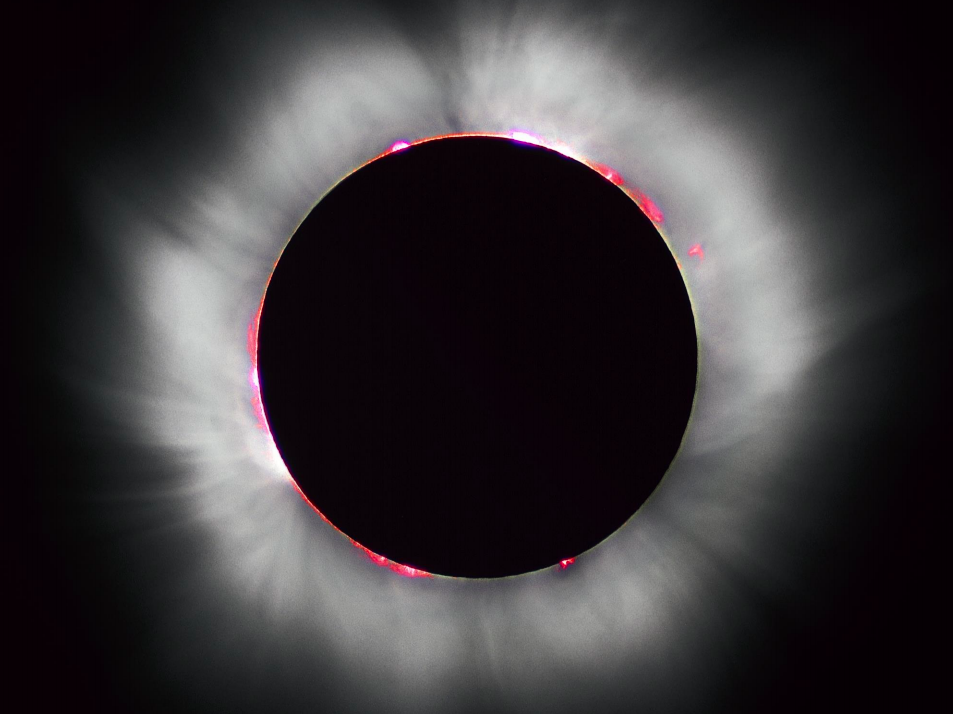
\includegraphics[width=0.5\textwidth]{poglavlja/7/slike/slika1.png}
\end{center}
\caption{Prikaz korona virusa}
\label{fig:pkv}
\end{figure}

\section{Transformacija matrice rastojanja u evolutivno stablo}
\label{sec:transformacijamatrice}

\subsection{Konstrukcija matrice rastojanja}
\label{subsec:matricarastojanja}

Na osnovu vi\v{s}estrukog poravnanja dobijamo matricu rastojanja iz koje \v{z}elimo da konstrui\v{s}emo evolutivno stablo.
Defini\v{s}imo najpre \v{s}ta predstavlja svaki element ove matrice:

\begin{definicija}
Jedan element matrice u oznaci $D_{i,j}$ predstavlja broj razli\v{c}itih simbola u \textit{i}-tom i \textit{j}-tom redu vi\v{s}estrukog poravnanja.
\end{definicija}

Na slici \ref{fig:pkmr} je prikazana konstrukcija matrice rastojanja.

\begin{figure}[h!]
\begin{center}
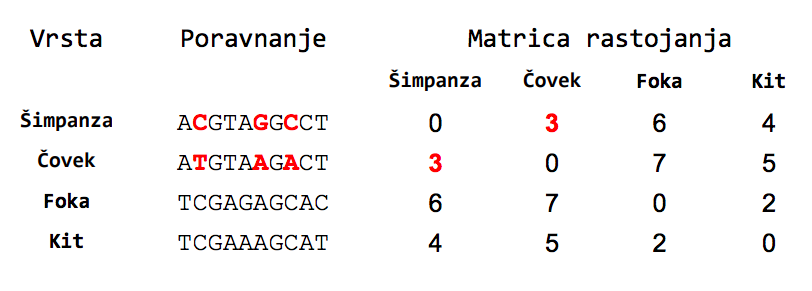
\includegraphics[width=0.75\textwidth]{poglavlja/7/slike/slika2.png}
\end{center}
\caption{Prikaz konstrukcije matrice rastojanja}
\label{fig:pkmr}
\end{figure}

\subsection{Stabla}
\label{subsec:stabla}

Stablo je povezani acikli\v{c}ni graf. Za povezana acikli\v{c}na stabla se mo\v{z}e pokazati:
\begin{itemize}
	\item Svako stablo sa bar dva \v{c}vora sadr\v{z}i bar dva lista.
	\item Svako stablo sa n \v{c}vorova sadr\v{z}i ta\v{c}no n - 1 grana.
\end{itemize}

U evolutivnom stablu listovi predstavljaju dana\v{s}nje vrste, dok unutra\v{s}nji \v{c}vorovi predstavljaju izumrle vrste. Koreni \v{c}vor predstavlja najdaljeg zajedni\v{c}kog predaka. Na slici \ref{fig:pmrioes} se mo\v{z}e videti primer evolutivnog stabla koji odgovara matrici.

\begin{figure}[h!]
\begin{center}
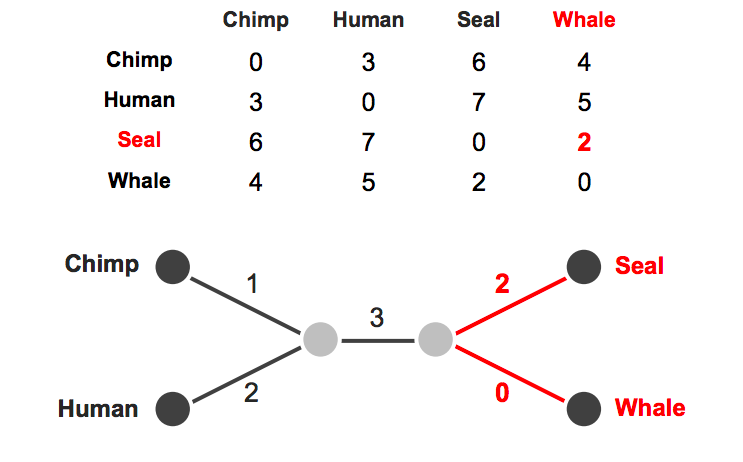
\includegraphics[width=0.75\textwidth]{poglavlja/7/slike/slika3.png}
\end{center}
\caption{Prikaz matrice rastojanja i njenog odgovaraju\'ceg evolutivnog stabla}
\label{fig:pmrioes}
\end{figure}

Uvodimo pojam rastojanja izme\dj u dva lista \textit{i} i \textit{j} u evolutivnom stablu u oznaci $d_{i, j}$:
\begin{tcolorbox}
\textbf{Problem izra\v{c}unavanja rastojanja izme\dj u listova:} Za dato te\v{z}insko stablo, izra\v{c}unati rastojanje izme\dj u listova.\\
\textbf{Ulaz}: Te\v{z}insko stablo sa n listova.\\
\textbf{Izlaz}: Matrica n x n ($d_{i, j}$), gde je $d_{i, j}$ du\v{z}ina putanje izme\dj u listova \textit{i} i \textit{j}.
\end{tcolorbox}

Ovaj problem je lako re\v{s}iv, zanima nas kako da za datu matricu rastojanja konstrui\v{s}emo evolutivno stablo. S obzirom na to da je mogu\'ce da iz jedne matrice dobijemo vi\v{s}e razli\v{c}itih stabala, neophodno je da matrice zadovoljavaju odre\dj ena svojstva, kako bi za jednu matricu dobili ta\v{c}no jedno stablo. Da bi to bilo mogu\'ce matrica mora biti aditivna.

Objasnicemo aditivne matrice kroz naredne definicije i teoreme:

\begin{definicija}
Za dato evolutivno stablo, matricu koja opisuje rastojanja izme\dj u njegovih listova zovemo \textit{aditivnom matricom}
\end{definicija}

\begin{teorema}
Matrica \textit{D} je aditivna akko za proizvoljna \v{c}etiri indeksa u matrici \textit{i, j} i \textit{k, l} va\v{z}i:

\begin{center}
\textit{$D_{ij}$ + $D_{kl}$ \textless= $D_{ik}$+$D_{jl}$ = $D_{il}$ + $D_{jk}$}
\end{center}

\end{teorema}

Na osnovu ove teoreme i definicije mo\v{z}emo zaklju\v{c}iti na koji na\v{c}in da pove\v{z}emo listove u evolutivnom stablu \ref{fig:pples}.

\begin{figure}[h!]
\begin{center}
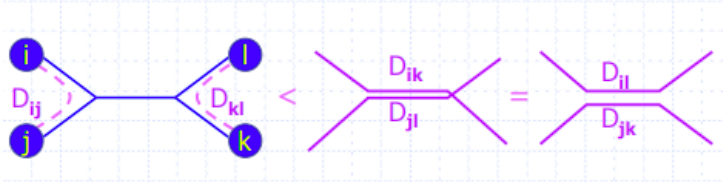
\includegraphics[width=0.75\textwidth]{poglavlja/7/slike/slika4.png}
\end{center}
\caption{Prikaz povezivanja listova u evolutivnom stablu}
\label{fig:pples}
\end{figure}

Po\v{s}to je za jednu matricu mogu\'ce konstruisati vi\v{s}e evolutivnih stabala, uvek je bolje izabrati prosto stablo. 

\begin{definicija}
\textbf{Prosto stablo:} stablo bez \v{c}vorova stepena \textgreater=2.
\end{definicija}

\begin{teorema}
Postoji ta\v{c}no jedno prosto stablo koje odgovara aditivnoj matrici.
\end{teorema}

Sada mo\v{z}emo formulisati \textbf{problem filogeneze na osnovu rastojanja}:

\begin{tcolorbox}
Konstruisati evolutivno stablo na osnovu aditivne matrice rastojanja. \\
\textbf{Ulaz:} Aditivna matrica rastojanja.\\
\textbf{Izlaz:} Prosto stablo koje odgovara datoj matrici rastojanja.
\end{tcolorbox}

\section{Prema algoritmu za rekonstrukciju filogenetskog stabla na osnovu rastojanja}
\label{pazrfsnor}

Primetimo da minimalna pozitivna vrednost matrice rastojanja odgovara listovima u stablu koje povezuje zajedni\v{c}ki roditelj. Takve listove nazivamo \textbf{susednim listovima}.\\

U primeru \ref{fig:psl} foka i kit su susedi (jer dele istog roditelja).

\begin{figure}[h!]
\begin{center}
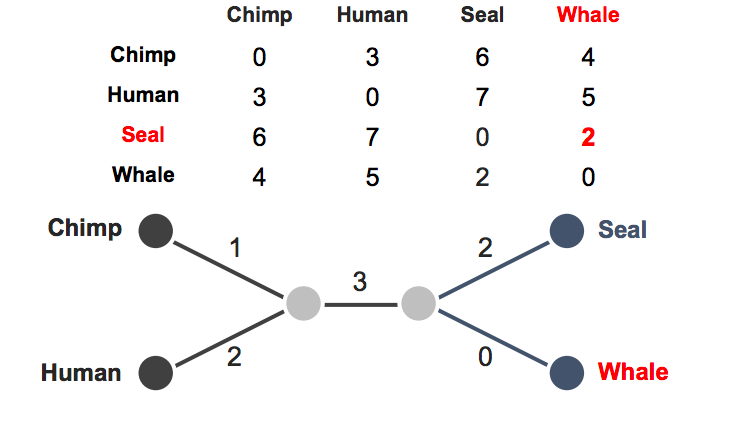
\includegraphics[width=0.75\textwidth]{poglavlja/7/slike/slika5.png}
\end{center}
\caption{Prikaz susednih listova}
\label{fig:psl}
\end{figure}

\begin{teorema}
Za svako prosto stablo sa bar dva \v{c}vora postoji bar jedan par susednih listova.
\end{teorema}
Dakle, mo\v{z}emo pretpostaviti da \'cemo uvek imati par susednih listova. Mi znamo da su \textit{kit} i \textit{foka} susedni listovi i da dele zajedni\v{c}kog roditelja, me\dj utim, ne znamo koja se vrednost pridru\v{z}uje svakoj od ovih grana. Da bismo dobili rastojanje izme\dj u susednih listova \textit{i} i \textit{j} od roditelja \textit{m} potrebno je da imamo jo\v{s} neki list unutar takvog stabla, recimo list \textit{k}. Razmatramo slede\'ca rastojanja: $d_{i,k}, d_{j, k}, d_{i,j}$ su rastojanja izme\dj u listova koja su data u matrici rastojanja, dok rastojanja $d_{i, m} i d_{j, m}$ koja predstavljaju rastojanja izme\dj u lista i unutra\v{s}njeg \v{c}vora, nisu data \ref{fig:filstab}.\\
Da bismo dobili rastojanje izme\dj u \v{c}ora \textit{i} i \v{c}vora \textit{j} treba da pratimo ljubi\v{c}asto i plavo rastojanje \ref{fig:filstab}. Sli\v{c}no ra\v{c}unamo i $d_{i, k}$ i $d_{j, k}$, a $d_{k, m}$ dobijamo sabiranjem kao na slici \ref{fig:filstab}. Sa velikim \textbf{D} ($D_{i, k}, D_{j, k}, D_{i, j}$) ozna\v{c}avamo elemente matrice rastojanja, dok sa malim \textbf{d} ozna\v{c}avamo rastojanje izme\dj u bilo koja dva \v{c}ora u evolutivnom stablu. \\
Kada znamo rastojanje od $d_{k,m}$ sada mo\v{z}emo da dobijemo $d_{i,m}$ kao: ($D_{i, k} + D_{i, j} – D_{j, k}$) / 2. Analogno dobijamo i za drugog suseda $d_{j, m}$.\\
Obratimo pa\v{z}nju da je \v{c}vor \textit{k} proizvoljan - bilo koji list koji je razli\v{c}it od listova \v{c}ija rastojanja do roditeljskog \v{c}vora tra\v{z}imo.\\

\begin{figure}[h!]
\begin{center}
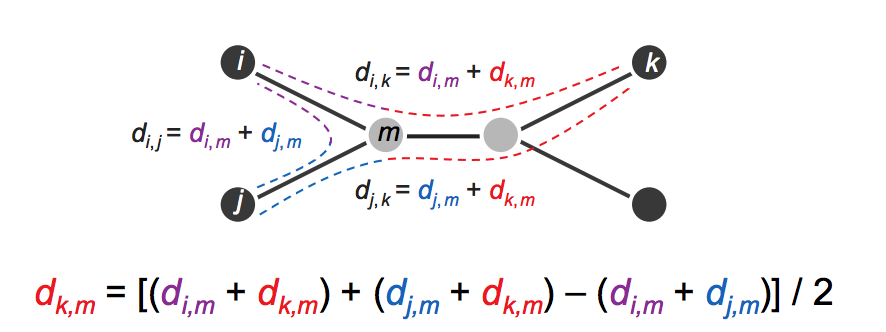
\includegraphics[width=0.7\textwidth]{poglavlja/7/slike/slika7.png}
\end{center}
\caption{Prikaz rekonstrukcije filogenetskog stabla na osnovu rastojanja}
\label{fig:filstab}
\end{figure}

Posmatrajmo sada opet evolutivno stablo. Foka \'ce biti \v{c}vor \textit{i}, \textit{j} \'ce biti susedan \v{c}vor kit. Za \textit{k} mo\v{z}emo uzeti po algoritmu, bilo koji \v{c}vor, biramo \v{s}impanzu. Sada va\v{z}i: 
\begin{center}
$d_{Seal, m} = (D_{Seal, Chimp} + D_{Seal, Whale} – D_{Whale, Chimp}) / 2$
\end{center}

Ovakav rekurzivni pristup \footnote{Ceo pristup, radi boljeg razumevanja, pogledati na slajdovima sa predavanja.} nije moguce primeniti za svaku matricu, u tim situacijama koristimo \textit{AdditivePhylogeny} algoritam.

\section{AdditivePhylogeny algoritam}
\label{addalg}

\begin{figure}[h!]
\begin{center}
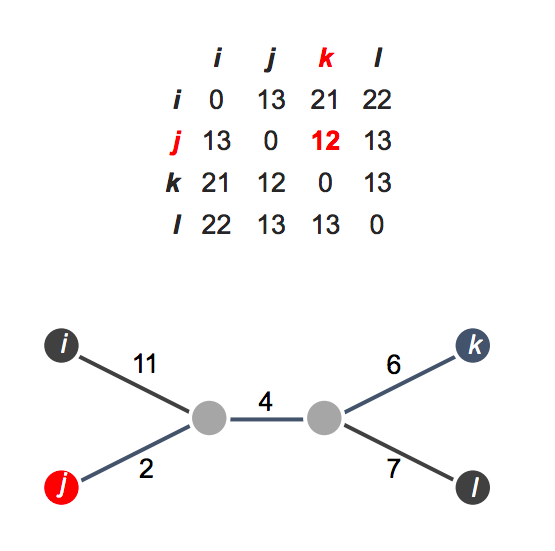
\includegraphics[width=0.5\textwidth]{poglavlja/7/slike/slika6.png}
\end{center}
\caption{Primer matrice za koju ne mo\v{z}emo primeniti prethodni pristup}
\label{fig:pmzknppp}
\end{figure}

Na slici \ref{fig:pmzknppp} mo\v{z}emo videti da je minimalni element $D_{j,k}$, a \textit{j} i \textit{k} nisu susedi, zato ne mo\v{z}emo primeniti prethodni pristup, iako je matrica ultrametri\v{c}na. Umesto tra\v{z}enja suseda, poku\v{s}ajmo da izra\v{c}unamo du\v{z}inu krajnjih grana, onih grana koje vode do listova. O du\v{z}inama spolnjih grana govori naredna teorema:

\begin{teorema}
\textbf{O du\v{z}ini spoljnih grana:} \textit{LimbLength(i)} je jednako minimalnoj vrednosti ($D_{i, k}$ + $D_{i, j}$ - $D_{j, k}$)/2 po svim listovima \textit{j} i \textit{k}.
\end{teorema}

Isklju\v{c}ujemo pretpostavku koju smo imali kod susednih listova, dakle ra\v{c}unamo rastojanje samo za jedan list, jer ne znamo koji joj je susedni \v{c}vor, pa zato uzimamo sve kombinacije za \textit{j} i \textit{k}. 

Prika\v{z}imo AdditivePhylogeny algoritam:

\begin{tcolorbox}
1. Izaberemo proizvoljno list, npr. \textit{j}. \\
2. Izra\v{c}unamo du\v{z}inu njegove krajnje grane, LimbLength(\textit{j}). \\
3.OduzmemoLimbLength(\textit{j}) od svake grane i dobijemo matricu \textit{$D^{bald}$}  u kojoj do lista \textit{j} vodi ogoljena (bold) grana (du\v{z}ine 0). \\
4. Uklonimo \textit{j}-ti red i kolonu iz matrice i dobijemo (n - 1) x (n - 1) matricu \textit{$D^{trim}$}. \\
5. Konstrui\v{s}emo Tree($D^{trim}$). \\
6. Identifikujemo ta\v{c}ku u Tree($D^{trim}$) gde list \textit{j} treba da se nalazi. \\
7. Dodamo list \textit{j} povezujuci ga granom du\v{z}ine LimbLength(\textit{j}) kako bismo formirali Tree(\textit{D}). 
\end{tcolorbox}

Ta\v{c}ka povezivanja za list \textit{j} je na putanji izme\dj u listova \textit{i} i \textit{k} na rastojanju $D^{bald}_{i, j}$ od \textit{i}. Dakle va\v{z}i: \textit{$D^{bald}_{i, j} + D^{bald}_{j, k} = D^{bald}_{i, k}$}.

Dobra strana ovog algoritma je da kreira stablo koje odgovara aditivnoj matrici, a lo\v{s}a da ne radi za neaditivne matrice \footnote{Za primer postupka pogledati slajdove sa predavanja}.
 
\section{Metod najmanjih kvadrata}
\label{sec:metodnajmanjihkvadrata}

U slu\v{c}aju da matrica nije aditivna, treba je aproksimirati nekom aditivnom matricom. Aproksimacija se vr\v{s}i na slede\'ci na\v{c}in:

\begin{tcolorbox}
\begin{center}
Discrepancy(T, D) = $\sum_{1 \leq i \textless j \leq n} (d_{i, j}(T) - D_{i, j})^{2}$
\end{center}
\end{tcolorbox}

Treba dodeliti du\v{z}ine granama u stablu T tako da veli\v{c}ina Discrepancy(T, D) bude minimalna.

U op\v{s}tem slu\v{c}aju, za stablo date topologije postoji algoritam polinomijalne slo\v{z}enosti koji \'ce dodeliti du\v{z}ine granama stabla tako da diskrepanca bude minimalna. Me\dj utim, u prakti\v{c}nim primenama ne\'ce biti poznata topologija stabla pa stoga moramo ra\v{c}unati minimum po svim mogu\'cim stablima. Sa dodavanjem svakog lista u stablo, broj razli\v{c}itih topologija stabala raste eksponencijalno. Problem minimizacije diskrepance po svim mogu\'cim stablima je NP kompletan. U nastavku, razmotri\'cemo dve heuristike za konstrukciju stabla na osnovu neaditivnih matrica.

\section{Ultrametri\v{c}na evolutivna stabla}
\label{sec:ues}

\subsection{Modelovanje specijacije}
\label{subsec:ms}

U prakti\v{c}nim primenama, istra\v{z}iva\v{c}i \v{c}esto pretpostavljaju da svaki unutra\v{s}nji \v{c}vor odgovara \textit{specijaciji} kada se jedna vrsta deli na dve.

\begin{definicija}
\textbf{Nekoreno binarno stablo:} svaki \v{c}vor je stepena 1 ili 3.
\end{definicija}

\begin{definicija}
\textbf{Koreno binarno stablo:} nekoreno binarno stablo sa korenom (stepena 2) postavljenom na jednoj od grana.
\end{definicija}

\subsection{Ultrametri\v{c}na stabla}
\label{subsec:us}

\begin{definicija}
\textbf{Molekularni sat:} dodeljuje starost svakom \v{c}voru u stablu (starost listova = 0).
\end{definicija}

\begin{definicija}
\textbf{Te\v{z}ine grana:} razlika u starosti \v{c}vorova koje povezuju.
\end{definicija}

\begin{definicija}
\textbf{Ultrametri\v{c}no stablo:} udaljenost od korena do bilo kog lista je ista i predstavlja starost korena.
\end{definicija}

\subsection{UPGMA: heuristi\v{c}ko klasterovanje}
\label{subsec:upgma}

\begin{tcolorbox}
1. Formirati klaster za svaku dana\v{s}nju vrstu. Svaki klaster sadr\v{z}i jedan list.\\
2. Na\'ci dva najbli\v{z}a klastera $C_1$ i $C_2$ na osnovu prose\v{c}nog rastojanja izme\dj u njihovih \v{c}lanova $D_{avg}(C_1, C_2)$ = $\sum_{i\ in\ C_1, j\ in\ C_2} D_{i, j} / \mid C_1 \mid \bullet \mid C_2 \mid $ gde $\mid C \mid$ ozna\v{c}ava broj elemenata u klasteru C.\\
3. Spojiti $C_1$ i $C_2$ u jedinstveni klaster C.\\
4. Formirati novi \v{c}vor za klaster i granama povezati ga za \v{c}vorovima. Postaviti starost \v{c}vora C na $D_{avg}$($C_1$, $C_2$)/2.\\
5. A\v{z}urirati matricu rastojanja tako \v{s}to ubacimo novi \v{c}vor, izbacimo \v{c}vorove koje on sadr\v{z}i i izra\v{c}unamo rastojanja kao prose\v{c}na rastojanja izme\dj u svaka dva para klastera.\\
6. Iteriramo dok ne do\dj emo do jednog klastera koji sadr\v{z}i sve vrste.
\end{tcolorbox}

Dobra strana ovog algoritma je da kreira stablo za svaku matricu, a lo\v{s}a da stablo ne mora da odgovara aditivnoj matrici.

\section{Neighbour-Joining teorema}
\label{sec:njt}

Za datu matricu rastojanja \textit{D} dimenzije \textit{n x n}, njena \textbf{neighbour-joining} matrica u oznaci \textit{D*} defini\v{s}e se kao:\\
\begin{center}
$D^*_{i, j}$ = (n - 2) $\bullet$ $D_{i, j}$ - $TotalDistance_D(i)$ - $TotalDistance_D(j)$
\end{center}

 gde je $TotalDistance_D(i)$ suma rastojanja od \textit{i} do svih ostalih listova.

\begin{teorema}
\textbf{Neighbour-joining:} ako je matrica \textit{D} aditivna, onda minimalni element matrice \textit{D*} odgovara susednom listu u stablu \textit{Tree(D)}.
\end{teorema}

\begin{tcolorbox}
1. Konstrui\v{s}emo neighbour-joining matricu D* na osnovu matrice D.\\
2. Na\dj emo minimalni element $D^*_{i, j}$ matrice D*.\\
3. Izra\v{c}unamo $\bigtriangleup_{i, j}$ = ($TotalDistance_d$(i) - $TotalDistance_d$(j)) / (n - 2).\\
4. Postavimo LimbLength(i) na 1/2($D_{i, j}$ + $\bigtriangleup_{i, j}$) i LimbLength(j) na 1/2($D_{i, j}$ + $\bigtriangleup_{i, j}$).\\
5. Formiramo matricu D' tako \v{s}to uklonimo \textit{i}-ti i \textit{j}-ti red/kolonu iz D i dodamo \textit{m}-ti red/kolonu tako da za svako k va\v{z}i $D_{k, m}$ = ($D_{i, k} + D_{j, k} - D_{i, j}$) / 2..\\
6. Primenimo \textit{NeighborJoining} rekurzivno na D' da dobijemo Tree(D').\\
7. Vratimo krajnje grane do \v{c}vorova \textit{i} i \textit{j} i dobijemo Tree(D).
\end{tcolorbox}

\subsection{Slabosti metoda zasnovanih na rastojanju}
\label{subsec:smznr}

Kada vi\v{s}estruko poravnanje zamenimo matricom rastojanja, gubimo informacije o sekvencama iz poravnanja. Zbog toga ne mo\v{z}emo da zaklju\v{c}imo kakva je sekvenca odgovarala vrstama iz unutra\v{s}njih \v{c}vorova.

\section{Rekonstrukcija stabla na osnovu karakteristika}
\label{sec:rsnok}

Pre oko pedeset godina, istra\v{z}iva\v{c}i su konstruisali filogenetska stabla na osnovu anatomsko-fiziolo\v{s}kih osobina organizama koje su nazvane \textbf{karakteristikama} \ref{fig:karakt}.

\begin{figure}[h!]
\begin{center}
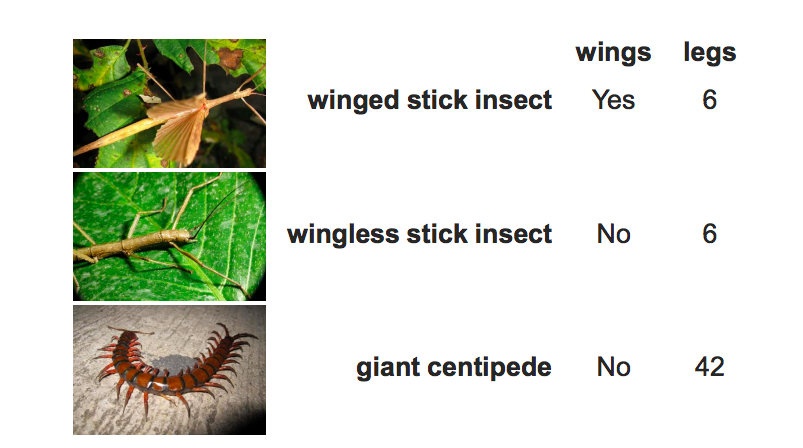
\includegraphics[width=0.7\textwidth]{poglavlja/7/slike/slika10.png}
\end{center}
\label{fig:karakt}
\end{figure}

\subsection{Filogeneza na osnovu karakteristika}
\label{subsec:fnok}

\begin{tcolorbox}
\textbf{Problem filogeneze zasnovane na karakteristikama:} Rekonstruisati evolutivno stablo na osnovu karakteristika. \\
Ulaz: Tabela karakteristika n x m za n vrsta i m karakteristika. \\
Izlaz: Stablo kog kog su vrste sa sli\v{c}nim karakteristikama blizu jedna drugoj. \\
\end{tcolorbox}

Kako bismo konstruisali evolutivno stablo na osnovu karakteristika?
Dolov zakon o nepovratnosti evolucionih procesa (1893): evolucija ne izmi\v{s}lja dva puta isti organ (npr. krila kod insekata).

\section{Problem male parsimonije}
\label{sec:pmp}

Skor parsimonije je suma Hamingovih rastojanja du\v{z} svake grane.

\begin{tcolorbox}
\textbf{Problem male parsimonije:} Odrediti oznake za unutra\v{s}nje \v{c}vorove korenog stabla. \\
Ulaz: Koreno binarno stablo gde je svaki list ozna\v{c}en jednim simbolom.\\
Izlaz: Oznake za sve ostale \v{c}vorove stabla takve da minimizuju skor parsimonije stabla.
\end{tcolorbox}

Algoritam dinami\v{c}kog programiranja: Neka je $T_v$ podstablo stabla T sa korenom u \v{c}voru v. Neka je $s_k(v)$ minimalni skor parsimonije stabla $T_v$ za sva mogu\'ca obele\v{z}avanja, pod pretpostavkom da je \v{c}vor v obele\v{z}en simbolom k. Minimalni skor parsimonije stabla jednak je minimalnoj vrednosti $s_k(root)$ po svim simbolima k. Neka je \textit{$\delta_{i, j}$} Kronekerov delta simbol:
\begin{itemize}
\item \textit{$\delta_{i, j}$} = 0 ako i = j
\item \textit{$\delta_{i, j}$} = 1 ina\v{c}e
\end{itemize}
Va\v{z}i slede\'ca rekurentna relacija:
\begin{tcolorbox}
$s_k(v) = min_{all\ symbols\ i} {s_i(Daughter(v)) + \delta_{i,k}} + min_{all\ symbols\ j} {s_j(Son(v)) + \delta_{j,k}}$
\end{tcolorbox}

\section{Problem velike parsimonije}
\label{sec:pvp}

\begin{tcolorbox}
\textbf{Problem velike parsimonije:} Za dati skup niski, na\'ci stablo \v{c}iji su listovi ozna\v{c}eni ovim niskama koje ima najmanji skor parsimonije. \\
Ulaz: Kolekcija niski jednake du\v{z}ine. \\
Izlaz: Koreno binarno stablo T koje minimizuje skor parsimonije po svim mogu\'cim korenim binarnim stablima \v{c}iji su listovi ozna\v{c}eni datim niskama.\\
Ovaj problem je NP-kompletan.
\end{tcolorbox}

\subsection{Pohlepna heuristika za veliku parsimoniju}
\label{phzvp}

Primetimo da uklanjanje jedne unutra\v{s}nje grane, grane koja povezuje dva unutra\v{s}nja \v{c}vora (zajedno sa \v{c}vorovima), dovodi do stvaranja \v{c}etiri podstabla (W, X, Y, Z) \ref{fig:pscp}.

\begin{figure}[h!]
\begin{center}
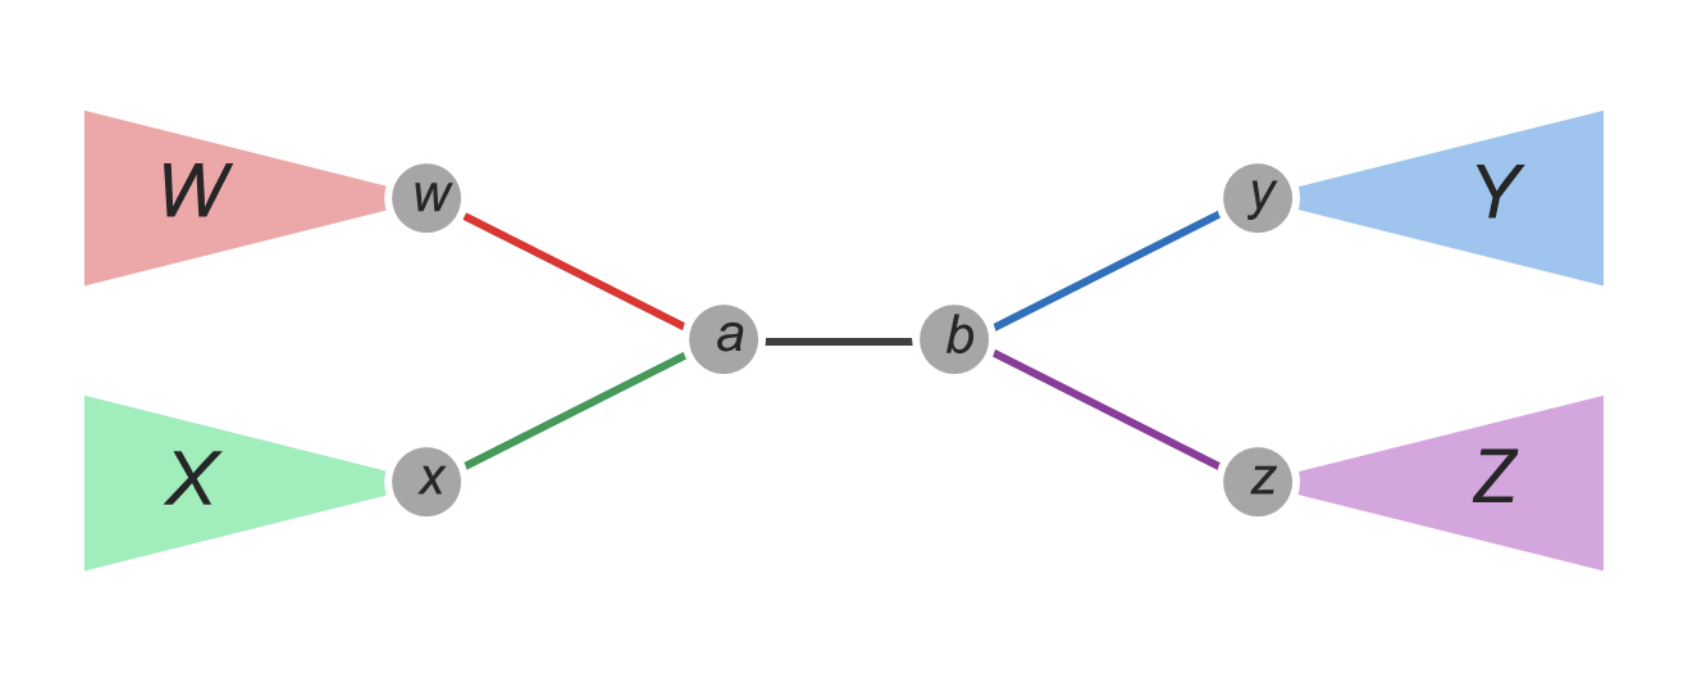
\includegraphics[width=0.7\textwidth]{poglavlja/7/slike/slika8.png}
\end{center}
\caption{Prikaz stvaranja \v{c}etiri podstabla}
\label{fig:pscp}
\end{figure}

Preure\dj enje rasporeda ovih stabala se naziva razmena najbli\v{z}ih suseda \ref{fig:psns}.

\begin{figure}[h!]
\begin{center}
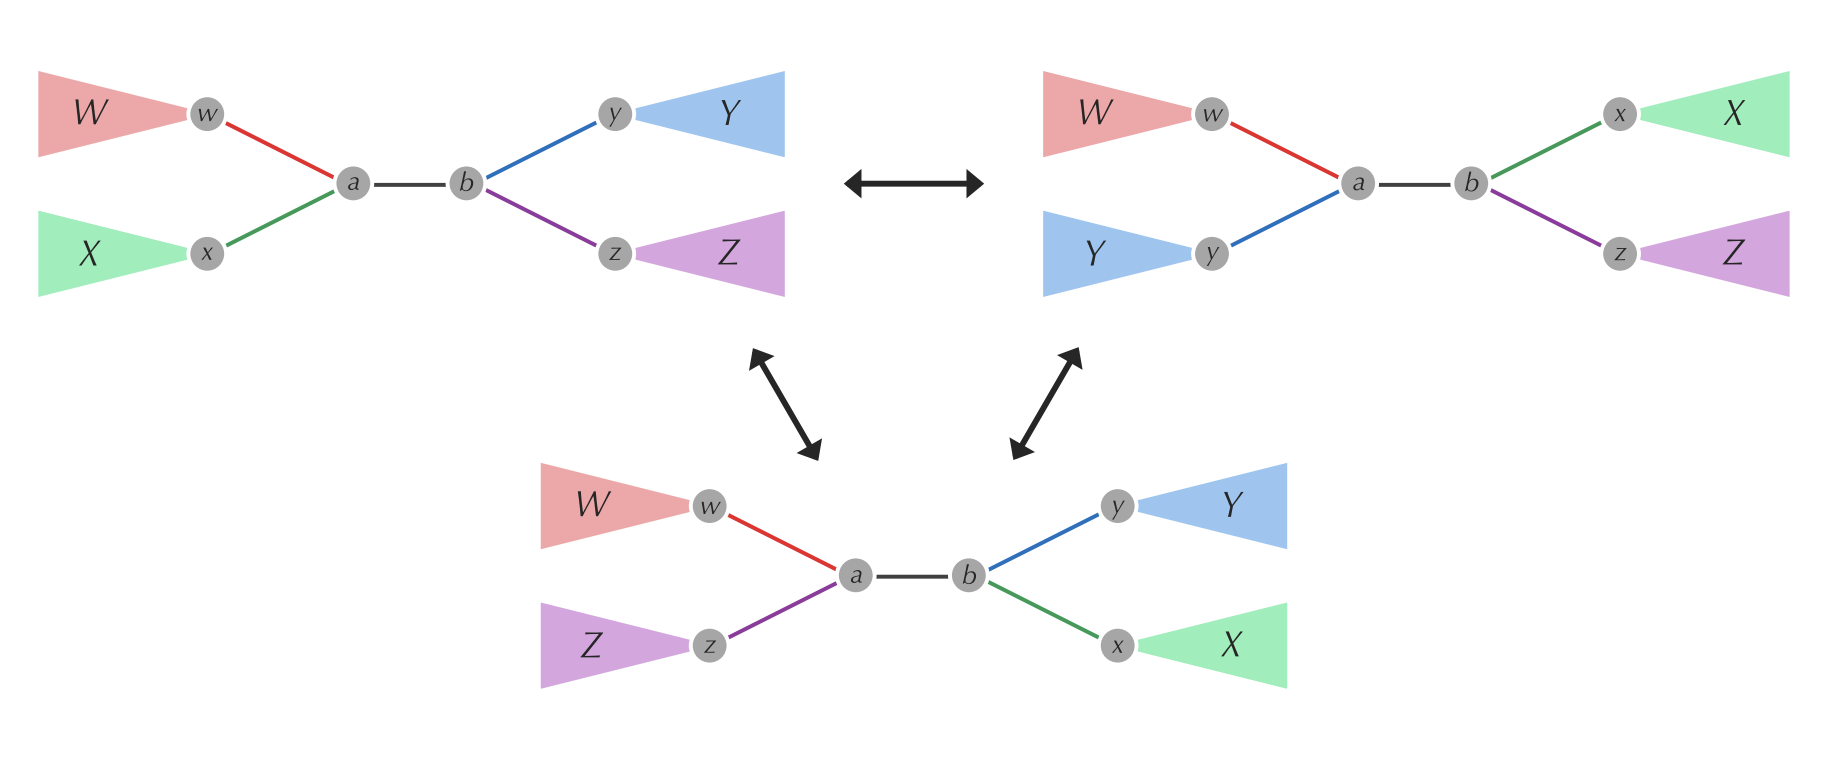
\includegraphics[width=0.7\textwidth]{poglavlja/7/slike/slika9.png}
\end{center}
\caption{Prikaz razmene najbli\v{z}ih suseda}
\label{fig:psns}
\end{figure}

\begin{tcolorbox}
\textbf{Problem najbli\v{z}ih suseda u stablu:} Za datu granu u binarnom stablu, generisati dva suseda ovog stabla. \\
Ulaz: Unutra\v{s}nja grana binarnog stabla.\\
Izlaz: Dva najbli\v{z}a suseda ovog stabla za datu unutra\v{s}nju granu.
\end{tcolorbox}

Heuristika za razmenu najbli\v{z}ih suseda:\\
1. Postaviti trenutno stablo na koreno binarno stablo proizvoljne strukture.\\
2. Pro\'ci kroz sve unutra\v{s}nje grane i izvr\v{s}iti sve mogu\'ce razmene najbli\v{z}ih suseda.\\
3. Re\v{s}iti problem male parsimonije za svako takvo stablo.\\
4. Ako stablo ima skor parsimonije bolje od optimalnog stabla, postaviti da to bude trenutno stablo; ina\v{c}e, vratiti trenutno stablo.

\newpage

\section{Zadaci sa vežbi}
\setexamplecodestyle

U nastavku će biti predstavljeni zadaci sa vežbi na kursu rađeni u programskom jeziku Python.

\subsection{Affine Gap Alignment}

\lstinputlisting[language=Python]{poglavlja/7/kodovi/1.py}


